\documentclass{beamer}
\usetheme{Singapore}
\usecolortheme{default}

\usepackage[utf8]{inputenc}
\usepackage[T1]{fontenc}
\usepackage{verbatim}
\usepackage{graphics}
\usepackage{listings}
\usepackage{lmodern}

\title{Understanding Git with Alloy}
\subtitle{Milestone 3}
\author{Cláudio Lourenço \and Renato Neves}
\institute{University of Minho\\
Formal Methods in Software Engineering}


\logo{ 
\includegraphics[width=0.15\textwidth]{images/csail_logo.png}
       
\includegraphics[width=0.15\textwidth]{images/uminho_eng_logo.png}}

\begin{document}

\frame {
   \titlepage
}

\frame{
   \frametitle{Table of contents}
   \tableofcontents 
}

\section{Git as VCS}

\begin{frame}
	\frametitle{Git as VCS}
	\begin{block}{Git is one of many Version Control Systems}
		\begin{itemize}
		\item Fast
		\item Efficient
		\item Oriented to snapshots, not differences
		\item Widely used
	\end{itemize}
	\end{block}
\end{frame}

\section{Project motivation and objectives}
\begin{frame}
	\frametitle{Motivation for this project}
	\begin{block}{Gap in the understanding of Git}
		\begin{itemize}
		\item Lack of precise descriptions
		\item Contradictions in some manuals
		\item Developers could benefit from a manual
		that is precise and rigorous
		\end{itemize}
	\end{block}
\end{frame}

\begin{frame}
	Quotation
\end{frame}

\begin{frame}
	\frametitle{Objectives of this project}
	\begin{block}{Shine some light in the dark world of Git}
		\begin{itemize}
			\item Build a precise model of how Git works
			\item Analyze the model
			\item Build a user manual based on specification a
			analysis 
		\end{itemize}
	\end{block}
\end{frame}


\section{Git internals}

\begin{frame}
   \frametitle{The Git Structure}
   \begin{figure}
      \centering
      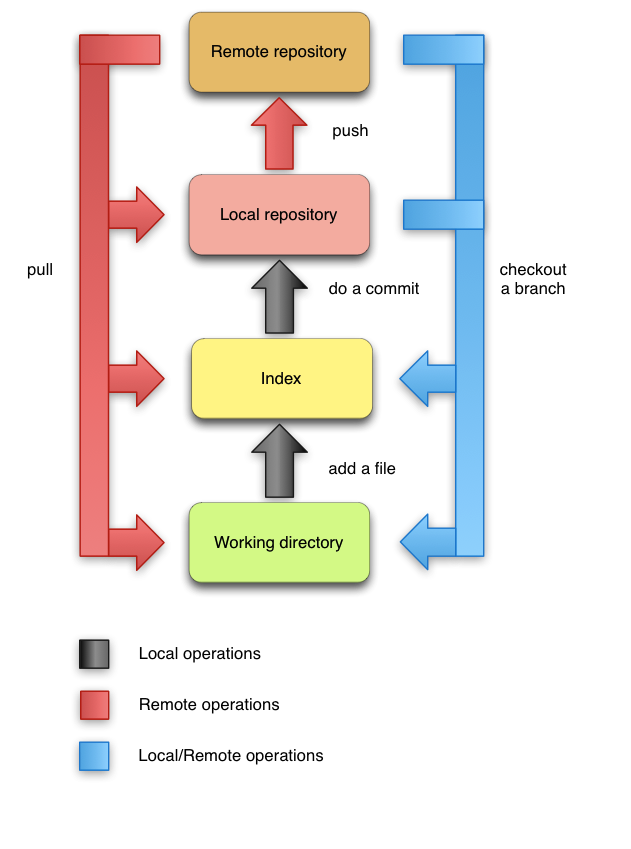
\includegraphics[width=0.5\textwidth]{images/git_workflow.png}
   \end{figure}
\end{frame}


\begin{frame}
\frametitle{Repository}
   \begin{figure}
      \centering
      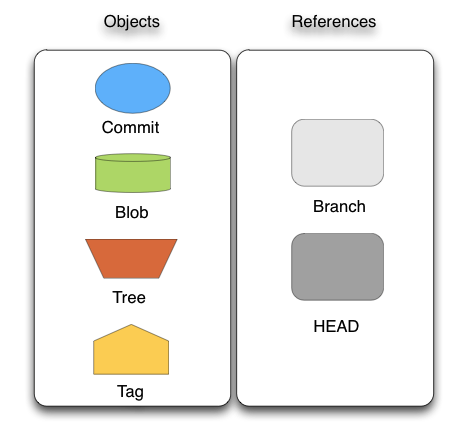
\includegraphics[width=0.5\textwidth]{images/legenda2.png}
   \end{figure}
\end{frame}

\begin{frame}[fragile]
   \frametitle{Blob and Tree}
   \begin{block}{Blob}
      \begin{itemize}
         \item Represents the content of a file;
         \item The name is calculated from its content;
      \end{itemize}
      \tiny
      \color{blue}
      \begin{lstlisting}
      sig Blob extends Object {}
      \end{lstlisting}
   \end{block}
   \begin{block}{Tree}
      \begin{itemize}
         \item Relation from names to Blobs or/and Trees;
         \item Used to represent the file system structure;
      \end{itemize}
      \tiny
      \color{blue}
      \begin{lstlisting}
      sig Tree extends Object {
         
         contains: Name -> lone(Tree+Blob)
      
      }
      \end{lstlisting}
   \end{block}
\end{frame}




\begin{frame}[fragile]
   \frametitle{Commit}
   \begin{itemize}
      \item It is like a snapshot of the project on a certain moment
      in time;
      \item Author, Committer, Comment - Not important for us;
      \item Parent - The Commit which originated the current;
      \item Tree - Pointer to a Tree Object;
   \end{itemize}
   \tiny
   \color{blue}
   \begin{lstlisting}
                        sig Commit extends Object {
                           points : Tree,
                           parent : set Commit,
                           abs: Path -> Object,
                           merge : set State
                        }
                           
                        sig RootCommit extends Commit {}
\end{lstlisting}
\end{frame}

\begin{frame}[fragile]
\frametitle{Branch and HEAD}
   \begin{block}{Branch}
      \begin{itemize}
         \item It is just a pointer to a commit;
      \end{itemize}
   \end{block}
   \begin{block}{HEAD}
      \begin{itemize} 
         \item Special reference that identifies the current Branch;
      \end{itemize}
   \end{block}
   \tiny
   \color{blue}
   \begin{lstlisting}
                        sig Branch{
                           marks: Commit lone -> State,
                           branches: set State,
                           head: set State
                        }

                        lone sig Master extends Branch{}
   \end{lstlisting}
\end{frame}

\begin{frame}
	\frametitle{Repository}
	\begin{figure}
		\centering
		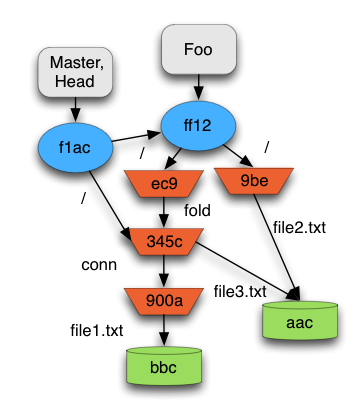
\includegraphics[width=0.5\textwidth]{images/object_assoc.png}
	\end{figure}
\end{frame}

\begin{frame}[fragile]
   \frametitle{Working Directory}
   \begin{itemize}
      \item Subset of a file system with the content of a project;
      \item These files can be the current files or files retrieved
      from the repository.
   \end{itemize}
   \tiny
   \color{blue}
   \begin{lstlisting}
                        sig Path {
                           pathparent: lone Path,
                           name: Name,
                           unmerge: set State
                        }

                        one sig Root extends Path{}
   \end{lstlisting}
\end{frame}

\begin{frame}[fragile]
   \frametitle{Index}
   \begin{itemize}
      \item Something in between the working directory and repository;
      \item It keeps a relation from file to content;
      \item The files in index will be in the next commit;
   \end{itemize}
   \vspace{10mm}
   \tiny
   \color{blue}
   \begin{lstlisting}
                        sig File{
                           path: Path,
                           blob: Blob,
                           index: set State
                        }

   \end{lstlisting}

\end{frame}


\section{Specification of operations}

\begin{frame}[fragile]
   \frametitle{Add}
   \begin{figure}
      \centering
      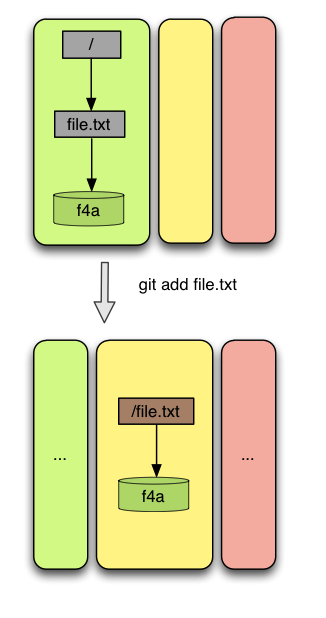
\includegraphics[width=0.3\textwidth]{images/add1.png}
   \end{figure}
\end{frame}

\begin{frame}[fragile]
   \frametitle{Remove}
   \begin{figure}
      \centering
      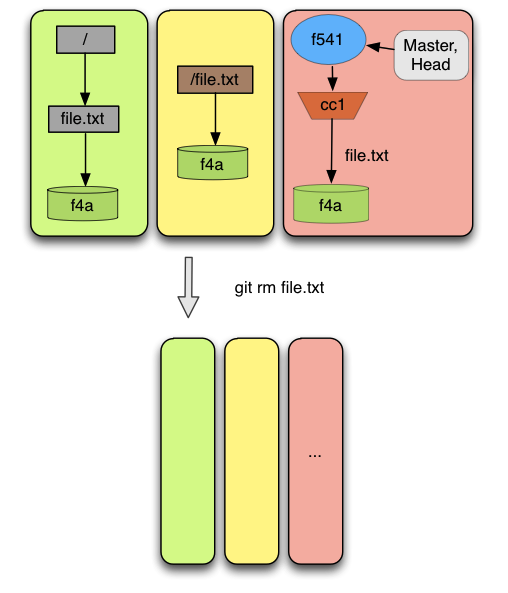
\includegraphics[width=0.45\textwidth]{images/remove1.png}
   \end{figure}
\end{frame}

\begin{frame}
	\frametitle{Commit}
\end{frame}

\begin{frame}
	\frametitle{Checkout}
\end{frame}

\begin{frame}
	\frametitle{Merge}
\end{frame}

\begin{frame}[fragile]
   \frametitle{Modeled Operations}
   \begin{itemize}
      \item Add and Remove
      \item Commit
      \item Branch and Branch Remove
      \item Checkout
      \item Merge (2-way and fast-forward)
   \end{itemize}
\end{frame}

\section{Documentation}

\begin{frame}
	\frametitle{Manual}
	\begin{block}{Built a manual that describes}
	\begin{itemize}
		\item Motivation for the manual
		\item Git internals
		\item Git operations
	\end{itemize}
	\end{block}
\end{frame}

\begin{frame}
	\frametitle{Website}
	\begin{itemize}
	\item Website created based on the manual 
	\item http://nevrenato.github.com/CSAIL\_Git
	\end{itemize}

\end{frame}

\section{Conclusion}

\begin{frame}
	\frametitle{Future Work}
	\begin{itemize}
	\item Model more operations 
		\begin{itemize}
			rebase, fetch, 3-way merge....
		\end{itemize}
	\item Specify more properties that the model does (not) guarantee
	\item Build interactive diagrams of concrete examples of operations 
	\end{itemize}
\end{frame}

\begin{frame}
	\frametitle{Conclusions}
\end{frame}


\end{document}
